\chapter{A look into the codes} \label{ch:lookinto}

In this chapter segments of the code will be explained.

\section{Include files} 

The compiler will always look through the first lines before doing anything else. This is why it is needed to include all the files that is wanted, in the code, in the first lines.\\

\begin{figure}[h]
\begin{center}
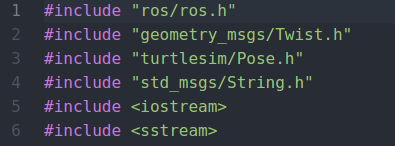
\includegraphics[width=.5\textwidth]{figures/therealinclude.png}
\caption{Include files}
\end{center}
\end{figure}\label{fig:include}

\begin{itemize}
\item \texttt{ros/ros.h}\\
This is a header to include all headers necessary for the common pieces in the ROS system.\\
\item \texttt{geometry\_msgs/Twist.h}\\
Includes the headers for the common geometrics as poses, vectors and points.\\
\item \texttt{turtlesim/pose.h}\\
This header file is only needed in the \texttt{Turtlesim\_mover}, since turtlesim/pose is a publisher.\\
This creates the headers for the pose of the virtual turtle.\\
\item \texttt{std\_msgs/String.h}\\
Is a automatized string header, which is generated from the String.msg file.\\
\item \texttt{<iostream>}\\
This is the input/output stream and helps with just that.\\
\item \texttt{<sstream>}\\
Include the std::stringstream.\\

\end{itemize}

\section{The node handler}
Before it is possible to use any ROS components their must be a initiation of ROS see first line \ref{fig:nodehandel}. The init needs 3 arguments argv, argc and a name in this it is called publish\_velocity. The nodehandle \ref{fig:nodehandel} on the second line,in need to initiate the node. The nodehandle is declared to be "n" in the mover node.
\begin{figure}[h]
\begin{center}
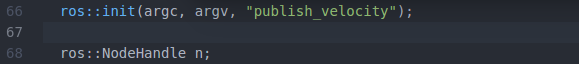
\includegraphics[width=.9\textwidth]{figures/nodehandel.png}
\caption{initiation of node-handle}
\end{center}
\end{figure}\label{fig:nodehandel}


\section{Publisher}
\begin{figure}[h]
\begin{center}
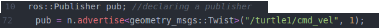
\includegraphics[width=.9\textwidth]{figures/publisher.png}
\caption{Publisher}
\end{center}
\end{figure}\label{fig:publihser}
The publisher needs to be declared as variable, it is done by the first line see \ref{fig:publihser}.The next line show what message that is published in this case a geometry::Twist and what topic it is published on /turtle1/cmd\_vel.


\section{Subscriber}
The subscriber has more or less the same syntax to be declared as a publisher see \ref{fig:subscriber}. The syntax is a bit different, in the matter it does not need to known what message it needs to listen for, but only on which topic it needs to subscribe to. In the case of of this sub it listens to that is published on the Commands topic, it can handle 1000 messages in a cue, is there more in the buffer they will be discarded. To access the subscriber there is the need for a function named chatterCallback, every time something is published on the topic Commands it will be written to the function named chatterCallback.

\begin{figure}[h]
\begin{center}

\includegraphics[width=.9\textwidth]{figures/subscriber.png}
\caption{subscriber}
\end{center}
\end{figure}\label{fig:subscriber}

\section{UI\_turtlesim\_mover}

Firstly the include files are introduced.\\
After the include files global parameters are set, such as:\\
\texttt{ros::Publisher pub1;}\\
\texttt{ros::Subscriber sub1;}\\
\texttt{string done;}\\
then a void function is made.\\

\begin{figure}[h]
\begin{center}
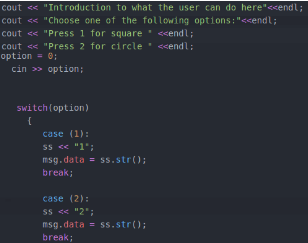
\includegraphics[width=.5\textwidth]{figures/switch.png}
\caption{VoidFunction of UI}
\end{center}
\end{figure}\label{fig:switch}

The void function as seen in \ref{fig:switch}, introduces a series of cout, which will print the text to the users screen.\\
Then the cin option appears. It will determine whether the user will press 1 or 2, and will then store the choice in "Option".\\
This leads to the next step in the code which is the switch. The switch, in this code, is used for the user to stay in the program. This gives the opportunity to user to stay in the program and give multiple commands to the publisher.\\
When storing the data "1" in the cin, the switch will then use the stored data to move it through case(1). When in case(1), the code will then send the data over a message string which will "talk" to the listener. Hereby the user can acknowledge that the turtlesim will react accordingly to the user input. Lastly the code will spinOnce and return to the main function.\\
After the nodehandle, publisher, main function, init:: and subscriber is set, see \ref{fig:publihser}, and \ref{fig:subscriber}, it will then go into a while loop.\\
\texttt{while(ros::ok())}\\
The code will now only break when the user closes the command "\^c", all nodehandles has been destroyed or the nodes are pushed off the internet.\\
While ros is okay, the for loop will then run, which means that if the expression inside the loop is true, then the loop will run until the expression is false. This loop is used for making a specific code run the desired times.\\
In the end it will make the loop spinOnce, and then return 0;\\



\section{Turtlesim\_mover}

\begin{figure}[h]
\begin{center}
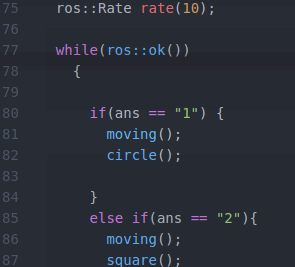
\includegraphics[width=.5\textwidth]{figures/while.png}
\end{center}
\end{figure}\label{fig:while}



\begin{figure}[h]
\begin{center}
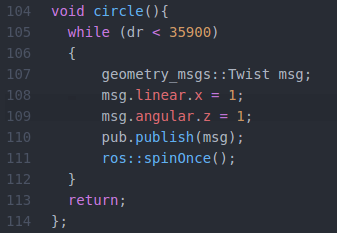
\includegraphics[width=.5\textwidth]{figures/void-circle.png}
\end{center}
\end{figure}\label{fig:void-circle}
